% Requires:
% \usepackage{pgfplots}
% \pgfplotsset{compat=1.18}
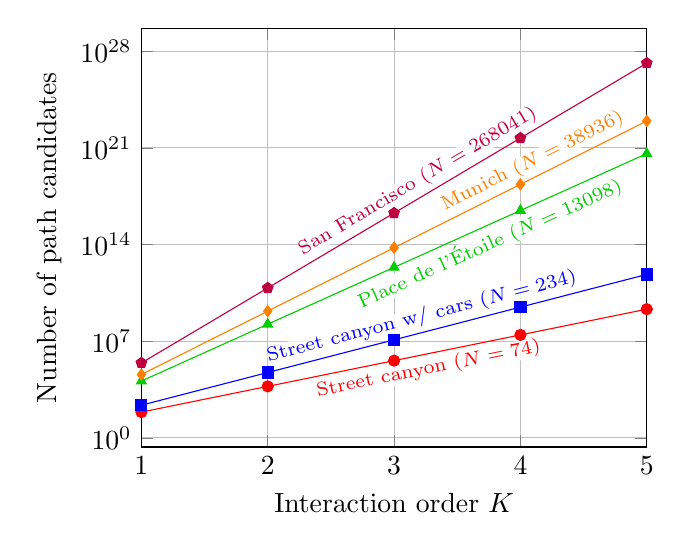
\begin{tikzpicture}
  \begin{axis}[
      width=8cm,
      ymode=log,
      xmin=1, xmax=5,
      xlabel={Interaction order $K$},
      ylabel={Number of path candidates},
      grid=major,
      % Define colors and markers for the 5 scenes
      cycle list={
        {red, mark=*},
        {blue, mark=square*},
        {green!80!black, mark=triangle*},
        {orange, mark=diamond*},
        {purple, mark=pentagon*},
      }
    ]
    \tikzset{mylabel/.style={font=\scriptsize, fill=white, fill opacity=0.8, text opacity=1, inner sep=0pt, outer sep=2pt, sloped, rounded corners}}

    % Scene: simple_street_canyon (N = 74)
    \addplot coordinates {
      (1,7.4000e+01) (2,5.4020e+03) (3,3.9435e+05) (4,2.8787e+07) (5,2.1015e+09)
      (6,1.5341e+11) (7,1.1199e+13) (8,8.1751e+14) (9,5.9678e+16) (10,4.3565e+18)
    } node[pos=0.25,below,mylabel] {Street canyon ($N=74$)};
    %\addlegendentry{Simple Street Canyon ($N=74$)}

    % Scene: simple_street_canyon_with_cars (N = 234)
    \addplot coordinates {
      (1,2.3400e+02) (2,5.4522e+04) (3,1.2704e+07) (4,2.9599e+09) (5,6.8967e+11)
      (6,1.6069e+14) (7,3.7441e+16) (8,8.7238e+18) (9,2.0327e+21) (10,4.7361e+23)
    } node[pos=0.25,above,mylabel] {Street canyon w/ cars ($N=234$)};
    %\addlegendentry{Street Canyon w/ Cars ($N=234$)}

    % Scene: etoile (N = 13098)
    \addplot coordinates {
      (1,1.3098e+04) (2,1.7154e+08) (3,2.2467e+12) (4,2.9425e+16) (5,3.8538e+20)
      (6,5.0474e+24) (7,6.6105e+28) (8,8.6578e+32) (9,1.1339e+37) (10,1.4851e+41)
    } node[pos=0.3,below,mylabel] {Place de l'Étoile ($N=13098$)};
    %\addlegendentry{Place de l'Étoile ($N=13098$)}

    % Scene: munich (N = 38936)
    \addplot coordinates {
      (1,3.8936e+04) (2,1.5160e+09) (3,5.9024e+13) (4,2.2981e+18) (5,8.9477e+22)
      (6,3.4838e+27) (7,1.3564e+32) (8,5.2812e+36) (9,2.0562e+41) (10,8.0060e+45)
    } node[pos=0.35,above,mylabel] {Munich ($N=38936$)};
    %\addlegendentry{Munich ($N=38936$)}

    % Scene: san_francisco (N = 268041)
    \addplot coordinates {
      (1,2.6804e+05) (2,7.1846e+10) (3,1.9258e+16) (4,5.1618e+21) (5,1.3836e+27)
      (6,3.7085e+32) (7,9.9403e+37) (8,2.6644e+43) (9,7.1416e+48) (10,1.9142e+54)
    } node[pos=0.25,above,mylabel] {San Francisco ($N=268041$)};
    %\addlegendentry{San Francisco ($N=268041$)}

  \end{axis}
\end{tikzpicture}
